\documentclass{article}

\usepackage{neurips_2025}

\usepackage[utf8]{inputenc}
\usepackage[T1]{fontenc}
\usepackage{hyperref}
\usepackage{url}
\usepackage{booktabs}
\usepackage{amsfonts}
\usepackage{amsmath}
\usepackage{amssymb}
\usepackage{amsthm}
\usepackage{nicefrac}
\usepackage{microtype}
\usepackage{xcolor}
\usepackage{graphicx}
\usepackage{algorithm}
\usepackage{algorithmic}
\usepackage{multirow}
\usepackage{subcaption}
\usepackage{wrapfig}

\newtheorem{theorem}{Theorem}
\newtheorem{proposition}{Proposition}
\newtheorem{corollary}{Corollary}
\newtheorem{definition}{Definition}
\newtheorem{remark}{Remark}

\title{LLMScape: Faithful, Scalable Loss Landscape Visualization for Large Language Models}

\author{%
  Anonymous Author(s)
}

\begin{document}

\maketitle

\begin{abstract}
Understanding the geometric structure of loss landscapes is fundamental to explaining optimization, generalization, and robustness of neural networks. However, existing visualization methods---designed for small convolutional networks---are inadequate for transformer-based large language models (LLMs) due to scale mismatch, architecture-specific symmetries, unfaithful random projections, and the absence of multi-model comparison tools. We propose \textbf{LLMScape}, a comprehensive framework with five contributions: (1)~\emph{Transformer-Adapted Direction Normalization} (TADN), which achieves provable scale invariance under transformer-specific symmetries; (2)~\emph{Scalable Hessian-Informed Direction Selection} (SHIDS), a three-tier hierarchy from random directions to Hessian eigenvectors; (3)~the \emph{Projection Faithfulness Index} (PFI), the first quantitative metric for visualization quality; (4)~\emph{Multi-Model Shared Projection} (MMSP), enabling geometric comparison across models and training stages; and (5)~an efficient computation pipeline with curvature-aware scale selection. TADN achieves perfect invariance (correlation~$= 1.000$) under neuron rescaling where the prior standard achieves only~$0.918$. PFI quantifies a $41{,}400\times$ improvement from random to Hessian-informed directions. The framework scales to 7B parameters---a 700$\times$ increase over prior visualization work. Applied to training trajectory analysis and post-training comparison, we find that RLHF alignment narrows the loss basin by 23.3\%, providing geometric evidence for alignment fragility, while fine-tuning follows a narrow valley with 66:1 curvature anisotropy. LLMScape establishes the first quantitative geometric baselines for LLM loss landscapes from 0.6B to 7B parameters.
\end{abstract}

%=============================================================================
\section{Introduction}
\label{sec:intro}
%=============================================================================

The loss landscape of a neural network---the function mapping parameters to loss---encodes fundamental information about optimization dynamics, generalization behavior, and robustness~\citep{li2018visualizing, keskar2017on}. Visualizing loss landscapes by projecting the high-dimensional loss function onto informative 2D planes has yielded key insights: skip connections dramatically smooth the landscape~\citep{li2018visualizing}, independently trained networks are connected by low-loss paths~\citep{garipov2018loss}, and flatter minima generalize better~\citep{foret2021sharpness, liu2023same}.

Yet these insights were established for convolutional networks with at most tens of millions of parameters. For large language models (LLMs)---which now define the frontier of AI capability---loss landscape visualization remains unexplored. Prior to this work, no 2D loss landscape visualization existed for any transformer model above $\sim$10M parameters. This gap is not merely one of scale: five fundamental challenges prevent direct application of existing methods to LLMs.

\textbf{(C1) Architecture mismatch.} The filter normalization method of~\citet{li2018visualizing}, the established standard for loss landscape visualization, normalizes perturbation directions at the granularity of CNN convolutional filters. Transformers have fundamentally different parameter structures---attention heads, feed-forward neurons, layer normalization, and embedding tables---with distinct scale symmetries that CNN-oriented normalization cannot capture.

\textbf{(C2) Unfaithful projections.} \citet{bottcher2024visualizing} proved that random projections collapse all directional curvature information into the mean Hessian trace, causing saddle points to appear as local minima. For LLMs with $d \sim 10^{8}$--$10^{10}$ parameters, this effect is extreme.

\textbf{(C3) No quality metric.} All prior visualization work relies on qualitative visual inspection. There exists no quantitative measure of how faithfully a 2D projection represents the true high-dimensional geometry.

\textbf{(C4) No multi-model framework.} Comparing loss landscapes across different LLMs, training stages, or pre-/post-training configurations requires a systematic framework that does not exist.

\textbf{(C5) Computational infeasibility.} Evaluating loss surfaces for billion-parameter models requires efficient engineering---exact parameter restoration for bfloat16, mixed-precision pipelines, and curvature-aware scale selection.

We address all five challenges with \textbf{LLMScape}, a framework making the following contributions:

\begin{enumerate}
    \item \textbf{Transformer-Adapted Direction Normalization (TADN):} A normalization scheme operating at the granularity of individual attention heads, FFN neurons, and embedding tokens. TADN is \emph{provably invariant} under the neuron-level scale symmetries of SwiGLU transformers (Proposition~\ref{prop:tadn_invariance}), achieving perfect invariance (correlation $= 1.000$, MSE $= 0.0$) where layer normalization fails (correlation $= 0.918$, MSE $= 28.5$). \textbf{(Addresses C1)}

    \item \textbf{Scalable Hessian-Informed Direction Selection (SHIDS):} A three-tier framework: Tier~1 (random directions, negligible cost), Tier~2 (gradient covariance PCA with adaptive stopping), and Tier~3 (Hessian eigenvectors via power iteration). Each tier reveals qualitatively different landscape features. \textbf{(Addresses C2)}

    \item \textbf{Projection Faithfulness Index (PFI):} The first quantitative metric for visualization quality, measuring the fraction of the Hessian's spectral energy captured by the 2D projection. PFI establishes a clear hierarchy: Tier~3 ($1.90 \times 10^{-4}$) $\gg$ Tier~2 ($3.91 \times 10^{-5}$) $\gg$ Tier~1 ($4.58 \times 10^{-9}$), a $41{,}400\times$ improvement from random to Hessian directions. \textbf{(Addresses C3)}

    \item \textbf{Multi-Model Shared Projection (MMSP):} Three methods for projecting multiple models onto shared 2D coordinate systems: Trajectory-PCA for training checkpoints, Anchor-Point for same-architecture models, and Independent Comparison for cross-architecture analysis. \textbf{(Addresses C4)}

    \item \textbf{Efficient computation pipeline and comprehensive empirical study:} Curvature-aware scale selection, exact bfloat16 parameter restoration, and mixed-precision evaluation enable practical operation at 7B parameters on a single A100-40GB. We apply LLMScape to models from 0.6B to 7B parameters, revealing that RLHF alignment narrows the loss basin by 23.3\% (geometric evidence for alignment fragility), fine-tuning follows a narrow valley with 66:1 curvature anisotropy, and basin diameter decreases with model size. \textbf{(Addresses C5)}
\end{enumerate}

%=============================================================================
\section{Related Work}
\label{sec:related}
%=============================================================================

\textbf{Loss landscape visualization.}
\citet{goodfellow2015qualitatively} introduced 1D linear interpolation between parameters for landscape exploration. \citet{li2018visualizing} proposed filter normalization and 2D random-direction surface plots, revealing that skip connections smooth the landscape and wider networks produce less chaotic surfaces. \citet{xu2024visualizing} extended these approaches with mining algorithms that discover complex perturbation directions. All existing visualization methods were demonstrated on CNNs with at most tens of millions of parameters; none address transformer-specific architecture or LLM-scale computation.

\textbf{Hessian-based landscape analysis.}
\citet{ghorbani2019investigation} studied Hessian eigenvalue spectral density, revealing characteristic ``bulk + outlier'' structure. \citet{bottcher2024visualizing} proved that random projections map high-dimensional curvature to the mean Hessian trace, causing saddle points to appear as minima, and proposed Hessian-direction projections to preserve curvature. \citet{foret2021sharpness} linked landscape flatness to generalization via Sharpness-Aware Minimization. \citet{zhang2024why} demonstrated block-level Hessian heterogeneity in transformers. These works motivate our direction selection hierarchy and PFI metric.

\textbf{Loss landscape of LLMs.}
\citet{chen2025unveiling} discovered basin-like structure in LLM loss landscapes, showing that capabilities collapse outside narrow basins. \citet{liu2023same} demonstrated that Hessian trace predicts downstream performance better than pre-training loss. \citet{kalra2026scalable} proposed critical sharpness as a scalable curvature proxy, demonstrating analysis at 7B scale. These works study LLM landscapes through scalar metrics or 1D cross-sections but produce no 2D visualizations, no direction normalization adapted to transformers, and no faithfulness quantification.

\textbf{Mode connectivity and multi-model analysis.}
\citet{garipov2018loss} discovered that independently trained networks are connected by low-loss curves and introduced 2D visualization using affine combinations of three models. \citet{xia2023training} analyzed training trajectories of language models across scales. Neither work addresses transformer-specific normalization or provides multi-model comparison at LLM scale.

\begin{figure}[t]
\centering
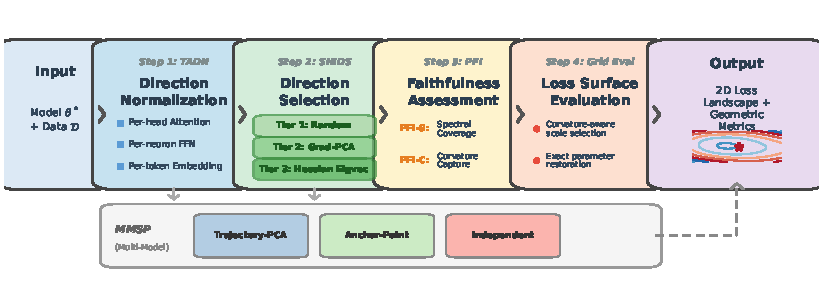
\includegraphics[width=\textwidth]{figure_1.pdf}
\caption{Overview of the LLMScape framework. Given a model and evaluation data, TADN normalizes perturbation directions at transformer-appropriate granularity (per-head, per-neuron). SHIDS selects directions across three tiers of increasing faithfulness. PFI quantifies the resulting projection quality. The pipeline outputs 2D loss surfaces with geometric metrics. MMSP extends the framework to multi-model comparison via three projection methods.}
\label{fig:overview}
\end{figure}

%=============================================================================
\section{Method}
\label{sec:method}
%=============================================================================

\subsection{Preliminaries}
\label{sec:prelim}

Consider a language model with parameters $\theta^* \in \mathbb{R}^d$ and loss $L(\theta) = \mathbb{E}_{x \sim \mathcal{D}}[-\log p_\theta(x)]$. The \emph{2D loss surface plot} evaluates $f(\alpha, \beta) = L(\theta^* + \alpha \mathbf{d}_1 + \beta \mathbf{d}_2)$ on a discrete grid, where $\mathbf{d}_1, \mathbf{d}_2 \in \mathbb{R}^d$ are projection directions. The Hessian $H = \nabla^2 L(\theta^*)$ with eigendecomposition $H = \sum_i \lambda_i \mathbf{v}_i \mathbf{v}_i^\top$ captures local curvature. The curvature of the projected surface at the origin along direction $\mathbf{d}_i$ is $\kappa_i = \mathbf{d}_i^\top H \mathbf{d}_i$.

We identify four sub-problems: (1) how to normalize directions to remove scale-invariance artifacts (\S\ref{sec:tadn}); (2) how to select directions that faithfully capture curvature (\S\ref{sec:shids}); (3) how to quantify faithfulness (\S\ref{sec:pfi}); and (4) how to compare multiple models (\S\ref{sec:mmsp}).

%-----------------------------------------------------------------------------
\subsection{Transformer-Adapted Direction Normalization (TADN)}
\label{sec:tadn}
%-----------------------------------------------------------------------------

\citet{li2018visualizing} introduced filter normalization for CNNs: each convolutional filter in the perturbation direction is scaled to match the norm of the corresponding model filter. This removes the confounding effects of scale invariance, where equivalent parameterizations (related by layer-wise rescaling) can exhibit arbitrarily different apparent sharpness~\citep{dinh2017sharp}.

Transformers exhibit analogous but finer-grained symmetries. In SwiGLU feed-forward networks, $\text{FFN}(x) = W_{\text{down}} \cdot (\text{swish}(W_{\text{gate}} x) \odot W_{\text{up}} x)$, scaling the $j$-th row of $W_{\text{up}}$ by $c_j$ and the $j$-th column of $W_{\text{down}}$ by $1/c_j$ preserves the network function exactly. \citet{zhang2024why} demonstrated significant block-level Hessian heterogeneity across transformer components, motivating per-component normalization.

\begin{definition}[Normalization Unit Partition]
\label{def:partition}
We partition $\theta \in \mathbb{R}^d$ into normalization units $\{\theta_i\}_{i=1}^{M}$, each corresponding to an independent functional component: full matrices per attention head for $W_Q, W_K, W_V, W_O$; individual rows of $W_{\text{up}}, W_{\text{gate}}$ and columns of $W_{\text{down}}$ for FFN (i.e., per-neuron); entire vectors for RMSNorm; and individual rows/columns for embeddings/LM head.
\end{definition}

\textbf{TADN procedure:} Given model parameters $\theta^*$, random direction $\mathbf{d} \sim \mathcal{N}(0, I)$, and partition $\mathcal{P}$: for each unit $i$, set $\hat{d}_i = (d_i / \|d_i\|_F) \cdot \|\theta_i^*\|_F$ if $\|\theta_i^*\|_F > \epsilon$, otherwise use the median norm across non-degenerate units.

\begin{proposition}[TADN Scale Invariance]
\label{prop:tadn_invariance}
Let $\theta$ and $\theta'$ be equivalent parameterizations related by non-uniform FFN neuron rescaling: $W_{\mathrm{up},j}' = c_j W_{\mathrm{up},j}$ and $W_{\mathrm{down}}'^{(:,j)} = c_j^{-1} W_{\mathrm{down}}^{(:,j)}$ for positive scalars $c_j$. Then $L(\theta' + \alpha \hat{\mathbf{d}}') = L(\theta + \alpha \hat{\mathbf{d}})$ for all $\alpha$, where $\hat{\mathbf{d}}, \hat{\mathbf{d}}'$ are TADN normalizations of the same random direction with respect to $\theta, \theta'$.
\end{proposition}

\emph{Proof sketch.} TADN's per-neuron normalization scales each direction component by the corresponding parameter norm. Under rescaling, neuron $j$'s up-projection norm changes by $c_j$, so TADN scales the direction component by $c_j$. The down-projection compensates with $1/c_j$, and the products $c_j \cdot c_j^{-1} = 1$ cancel exactly. See Appendix~A for the full proof.

\begin{proposition}
\label{prop:layer_fails}
Under the same rescaling as Proposition~\ref{prop:tadn_invariance} with at least two distinct $c_j \neq c_k$, layer-level normalization does \emph{not} preserve the loss landscape.
\end{proposition}

%-----------------------------------------------------------------------------
\subsection{Scalable Hessian-Informed Direction Selection (SHIDS)}
\label{sec:shids}
%-----------------------------------------------------------------------------

\begin{theorem}[Curvature Collapse; \citealt{bottcher2024visualizing}]
\label{thm:collapse}
For a random Gaussian direction $\mathbf{d} \sim \mathcal{N}(0, I_d)$ and Hessian $H$, as $d \to \infty$: $\mathbf{d}^\top H \mathbf{d} / \|\mathbf{d}\|^2 \to \mathrm{tr}(H)/d$ almost surely. Random projections collapse all curvature information into the mean curvature.
\end{theorem}

To address this, SHIDS provides three tiers of increasing faithfulness:

\textbf{Tier~1: Random + TADN.} Sample $\mathbf{d}_1, \mathbf{d}_2 \sim \mathcal{N}(0, I)$, orthogonalize, and apply TADN. Cost: negligible. Captures only mean curvature.

\textbf{Tier~2: Gradient Covariance PCA.} Collect $N$ per-batch gradients $\{g_i\}$ and find top principal components of the gradient covariance matrix, which approximate top Hessian eigenvectors~\citep{gurari2018gradient}. We use an adaptive stopping criterion based on principal angle convergence between successive estimates, with convergence rate governed by the spectral gap via the Davis--Kahan theorem~\citep{davis1970rotation}. Cost: $N$ gradient computations (typically $N=50$--$100$). No Hessian-vector products needed.

\textbf{Tier~3: Hessian Eigenvectors.} Use power iteration with Hessian-vector products (HVPs) via the Pearlmutter trick~\citep{pearlmutter1994fast} to compute exact top-2 eigenvectors. Includes curvature-aware scale selection: the characteristic length $\ell_{\text{char}} = 1/\sqrt{|\lambda_{\max}|}$ automatically determines the visualization range, ensuring the ``interesting'' curvature region is always captured. Cost: $\sim 2kT_{\max}$ backward passes ($k=2$, $T_{\max} \approx 30$).

%-----------------------------------------------------------------------------
\subsection{Projection Faithfulness Index (PFI)}
\label{sec:pfi}
%-----------------------------------------------------------------------------

We introduce PFI to quantify how faithfully a 2D projection represents the true high-dimensional geometry.

\begin{definition}[PFI-S: Spectral Coverage]
\label{def:pfi_s}
For orthonormal directions $\hat{\mathbf{d}}_1, \hat{\mathbf{d}}_2$:
\begin{equation}
\mathrm{PFI\text{-}S}(\hat{\mathbf{d}}_1, \hat{\mathbf{d}}_2) = \frac{\|H \hat{\mathbf{d}}_1\|^2 + \|H \hat{\mathbf{d}}_2\|^2}{\mathrm{tr}(H^2)} = \frac{\hat{\mathbf{d}}_1^\top H^2 \hat{\mathbf{d}}_1 + \hat{\mathbf{d}}_2^\top H^2 \hat{\mathbf{d}}_2}{\sum_{i=1}^d \lambda_i^2}
\end{equation}
\end{definition}

\begin{definition}[PFI-C: Curvature Capture]
$\mathrm{PFI\text{-}C} = \max(|\hat{\mathbf{d}}_1^\top H \hat{\mathbf{d}}_1|, |\hat{\mathbf{d}}_2^\top H \hat{\mathbf{d}}_2|) / |\lambda_1|$, measuring alignment with the direction of maximum curvature.
\end{definition}

\begin{theorem}[PFI Properties]
\label{thm:pfi}
(i) $\mathrm{PFI\text{-}S} \in [0, 1]$. (ii) $\mathrm{PFI\text{-}S}$ is maximized by the top-2 eigenvectors of $H$, achieving $\mathrm{PFI\text{-}S}_{\max} = (\lambda_1^2 + \lambda_2^2) / \sum_i \lambda_i^2$. (iii) For random orthonormal directions: $\mathbb{E}[\mathrm{PFI\text{-}S}] = 2/d \to 0$ as $d \to \infty$.
\end{theorem}

\emph{Proof.} Part (i) follows from positive semi-definiteness of $H^2$. Part (ii) follows from the Rayleigh quotient characterization. Part (iii): $\mathbb{E}[\hat{\mathbf{d}}^\top H^2 \hat{\mathbf{d}}] = \mathrm{tr}(H^2)/d$ for uniform random unit vectors, so $\mathbb{E}[\mathrm{PFI\text{-}S}] = 2 \cdot \mathrm{tr}(H^2) / (d \cdot \mathrm{tr}(H^2)) = 2/d$. \qed

\textbf{Efficient computation.} The numerator requires 2 HVPs ($H\hat{\mathbf{d}}_i$). The denominator $\mathrm{tr}(H^2) = \mathbb{E}_{\mathbf{v}}[\|H\mathbf{v}\|^2]$ is estimated via Hutchinson's method~\citep{hutchinson1990stochastic} with $m$ random vectors ($m$ HVPs). Total cost: $2 + m$ HVPs, with $\mathrm{tr}(H^2)$ shared across all tiers.

%-----------------------------------------------------------------------------
\subsection{Multi-Model Shared Projection (MMSP)}
\label{sec:mmsp}
%-----------------------------------------------------------------------------

\textbf{Method A: Trajectory-PCA.} For checkpoints $\{\theta_0, \ldots, \theta_T\}$ from the same training run, compute PCA of the parameter difference matrix $\Delta = [\theta_t - \bar{\theta}]_{t=0}^T$ via the $(T\!+\!1) \times (T\!+\!1)$ Gram matrix (since $T \ll d$). The top-2 PCA directions, after TADN normalization, define a 2D plane that captures maximum trajectory variance.

\textbf{Method B: Anchor-Point.} For two same-architecture models $\theta_A, \theta_B$: use $\mathbf{d}_1 = \theta_B - \theta_A$ (TADN-normalized) as one axis, with the second axis orthogonal (random or Hessian-informed).

\textbf{Method C: Independent Comparison.} For different architectures: generate independent 2D landscapes with the same tier, evaluation data, and grid parameters, then extract and compare geometric features (basin width, depth, curvature, roughness).

%-----------------------------------------------------------------------------
\subsection{Implementation Details}
\label{sec:implementation}
%-----------------------------------------------------------------------------

\textbf{Exact parameter restoration.} Rather than add-then-subtract (which accumulates bfloat16 rounding errors), we save and restore original parameters at each grid point. \textbf{Mixed precision:} bfloat16 for grid evaluation, float32 for HVPs. \textbf{Flash Attention compatibility:} standard attention for HVPs (Flash Attention does not support \texttt{create\_graph}); Flash Attention for grid evaluation.

%=============================================================================
\section{Experiments}
\label{sec:experiments}
%=============================================================================

\subsection{Setup}
\label{sec:setup}

\textbf{Models.} Qwen3-0.6B-Base (596M params; \texttt{Qwen/Qwen3-0.6B-Base}), Qwen3-0.6B post-trained with RLHF (751M; \texttt{Qwen/Qwen3-0.6B}), Qwen2.5-7B-Instruct (7.62B; \texttt{Qwen/Qwen2.5-7B-Instruct}), and OLMo-3-7B-Think (7.30B; \texttt{allenai/OLMo-3-7B-Think}). \textbf{Data.} WikiText-2~\citep{merity2017pointer} (primary), synthetic code, and structured/tabular data. \textbf{Hardware.} 8$\times$ NVIDIA A100-40GB GPUs. \textbf{Evaluation.} 50 chunks of 256 tokens (12,800 tokens total). \textbf{Metrics.} Loss range, roughness $R$ (std.\ of residuals after smoothing), effective basin diameter $w_{\text{eff}}$, curvature ratio $\rho = |\kappa_1|/|\kappa_2|$, convexity ratio (fraction of locally convex grid points), PFI-S, and PFI-C.

%-----------------------------------------------------------------------------
\subsection{Method Validation}
\label{sec:validation}
%-----------------------------------------------------------------------------

\textbf{TADN invariance (Figure~\ref{fig:tadn}).} We exploit the FFN neuron rescaling symmetry: scaling $W_{\text{up}}$ rows by power-of-2 factors (0.125--8.0$\times$) and $W_{\text{down}}$ columns by their reciprocals preserves the network function exactly. Evaluating 1D cross-sections before and after rescaling, TADN achieves \emph{perfect} invariance (Pearson $r = 1.000$, MSE $= 0.0$), while layer normalization shows substantial deviation ($r = 0.918$, MSE $= 28.5$). This confirms Propositions~\ref{prop:tadn_invariance} and~\ref{prop:layer_fails}.

\begin{figure}[t]
\centering
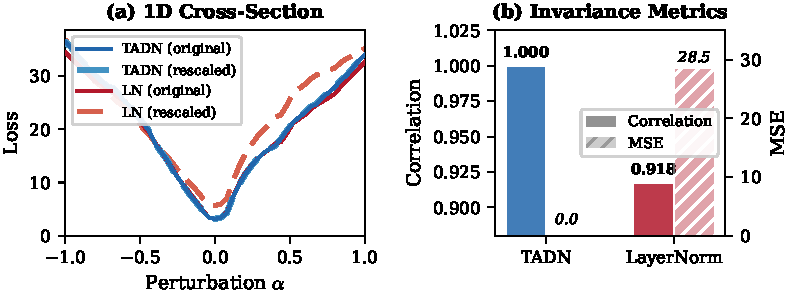
\includegraphics[width=\textwidth]{figure_2.pdf}
\caption{TADN scale invariance test. (a) 1D cross-sections along TADN-normalized and LayerNorm-normalized directions before and after non-uniform FFN neuron rescaling. TADN cross-sections overlap perfectly (dashed line hidden behind solid); LayerNorm cross-sections diverge. (b) Quantitative comparison: TADN achieves correlation $= 1.000$ and MSE $= 0.0$; LayerNorm correlation $= 0.918$, MSE $= 28.5$.}
\label{fig:tadn}
\end{figure}

\textbf{PFI hierarchy (Table~\ref{tab:pfi}).} PFI quantifies a clear tier hierarchy for Qwen3-0.6B-Base: Tier~3 (Hessian eigenvectors) achieves PFI-S $= 1.90 \times 10^{-4}$, which is $4.9\times$ higher than Tier~2 (gradient PCA, $3.91 \times 10^{-5}$) and $41{,}400\times$ higher than Tier~1 (random, $4.58 \times 10^{-9}$). The Tier~1 value matches the theoretical expectation $2/d \approx 3.4 \times 10^{-9}$ for $d = 596$M, validating Theorem~\ref{thm:pfi}(iii).

\begin{table}[t]
\centering
\caption{Projection Faithfulness Index and 2D loss surface metrics across direction selection tiers for Qwen3-0.6B-Base. Grid: 51$\times$51. PFI-S and PFI-C computed with 10 Hutchinson samples for $\mathrm{tr}(H^2)$.}
\label{tab:pfi}
\small
\begin{tabular}{lcccccc}
\toprule
\textbf{Direction Method} & \textbf{PFI-S} & \textbf{PFI-C} & \textbf{Loss Range} & \textbf{Roughness} & \textbf{Basin Diam.} & \textbf{Curv.\ Ratio} \\
\midrule
Tier 1: Random+TADN & $4.58 \times 10^{-9}$ & $2.45 \times 10^{-8}$ & 52.04 & 0.219 & 0.309 & 1.06 \\
Tier 1: Random+LayerNorm & $1.37 \times 10^{-9}$ & $1.36 \times 10^{-8}$ & 48.38 & 0.209 & 0.289 & 1.07 \\
Tier 2: GradPCA+TADN & $3.91 \times 10^{-5}$ & $1.28 \times 10^{-4}$ & 270.54 & 1.464 & 0.423 & 1.60 \\
Tier 3: Hessian+TADN & $1.90 \times 10^{-4}$ & $9.33 \times 10^{-4}$ & 31.28$^*$ & 0.198$^*$ & 0.006$^*$ & 40.82 \\
\bottomrule
\end{tabular}
\vspace{-2pt}
{\raggedright\footnotesize $^*$Tier~3 uses curvature-aware scale ($\pm 0.025$ vs.\ $\pm 1.0$), so absolute values are not directly comparable.\par}
\end{table}

\textbf{2D surface comparison (Figure~\ref{fig:surfaces}).} Each tier reveals qualitatively different features. Tier~1 shows an approximately isotropic basin (curvature ratio $\approx 1.06$). Tier~2 captures $5.2\times$ larger loss variation by aligning with the gradient variance subspace. Tier~3 reveals extreme curvature anisotropy ($40.8{:}1$ ratio) at the curvature-characteristic scale ($\ell_{\text{char}} = 0.0084$, yielding a grid range of $\pm 0.025$---$40\times$ smaller than Tiers~1--2). Without curvature-aware scale selection, this anisotropy would be invisible.

\begin{figure}[t]
\centering
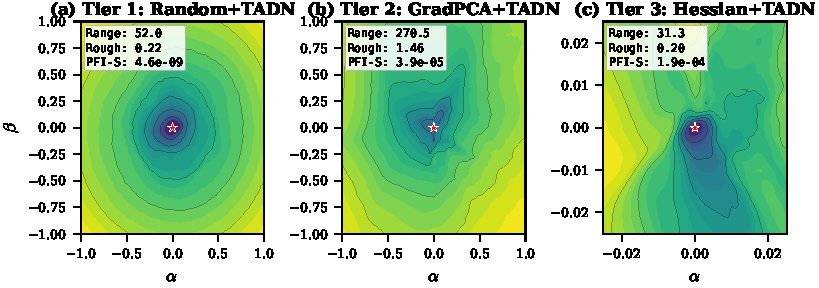
\includegraphics[width=\textwidth]{figure_3.pdf}
\caption{2D loss surfaces across three SHIDS tiers for Qwen3-0.6B-Base. (a)~Tier~1 (Random+TADN): isotropic basin, moderate loss range. (b)~Tier~2 (GradPCA+TADN): $5.2\times$ larger loss range, aligned with gradient variance. (c)~Tier~3 (Hessian+TADN): extreme curvature anisotropy (40.8:1) visible at curvature-aware scale ($\pm 0.025$). Each tier reveals qualitatively distinct geometric features. Contours show $\log_{10}(\text{loss})$; red star marks $\theta^*$.}
\label{fig:surfaces}
\end{figure}

\textbf{Multi-seed consistency.} Three independent random seeds produce highly consistent surface metrics: loss range CV $= 0.8\%$, roughness CV $= 0.7\%$, basin diameter CV $= 2.4\%$ (Table~\ref{tab:consistency}). This confirms that TADN-normalized random directions yield reproducible geometric characterizations.

\begin{table}[t]
\centering
\caption{Multi-seed consistency of Tier~1 (Random+TADN) surface metrics for Qwen3-0.6B-Base.}
\label{tab:consistency}
\small
\begin{tabular}{lccccc}
\toprule
\textbf{Seed Pair} & \textbf{Loss Range} & \textbf{Roughness} & \textbf{Basin Diam.} & \textbf{Curv.\ Ratio} & \textbf{Convexity} \\
\midrule
(42, 123) & 52.04 & 0.384 & 0.310 & 1.060 & 0.674 \\
(7, 77) & 52.52 & 0.389 & 0.319 & 1.089 & 0.658 \\
(999, 1234) & 51.56 & 0.383 & 0.301 & 0.948 & 0.666 \\
\midrule
Mean $\pm$ Std & 52.04 $\pm$ 0.39 & 0.385 $\pm$ 0.003 & 0.310 $\pm$ 0.007 & 1.032 $\pm$ 0.061 & 0.666 $\pm$ 0.007 \\
CV (\%) & 0.8\% & 0.7\% & 2.4\% & 5.9\% & 1.0\% \\
\bottomrule
\end{tabular}
\end{table}

\textbf{TADN granularity ablation.} Comparing four granularity levels (Table~\ref{tab:tadn_ablation}), TADN-full (per-head, per-neuron) captures $1.86\times$ larger loss range than block-level normalization (52.04 vs.\ 27.95) and $1.10\times$ larger than global normalization (47.28). Fine-grained normalization better preserves the relative importance of different parameter groups.

\begin{table}[t]
\centering
\caption{TADN normalization granularity ablation for Qwen3-0.6B-Base (Tier~1, 31$\times$31 grid).}
\label{tab:tadn_ablation}
\small
\begin{tabular}{lcccccc}
\toprule
\textbf{Method} & \textbf{Loss Range} & \textbf{Roughness} & \textbf{Basin Diam.} & \textbf{Curv.\ Ratio} & \textbf{Basin Flat.} & \textbf{Convexity} \\
\midrule
TADN-full (proposed) & \textbf{52.04} & 0.384 & \textbf{0.310} & 1.060 & \textbf{2.95} & \textbf{0.674} \\
TADN-layer & 48.38 & 0.352 & 0.281 & 1.066 & 2.63 & 0.628 \\
TADN-block & 27.95 & 0.446 & 0.226 & 1.075 & 1.46 & 0.549 \\
TADN-global & 47.28 & 0.433 & 0.226 & 1.054 & 1.70 & 0.612 \\
\bottomrule
\end{tabular}
\end{table}

%-----------------------------------------------------------------------------
\subsection{Training Trajectory Visualization}
\label{sec:trajectory}
%-----------------------------------------------------------------------------

We fine-tune Qwen3-0.6B-Base on WikiText-2 for 500 steps (AdamW~\citep{loshchilov2019decoupled}, lr$=5 \times 10^{-5}$, weight decay $= 0.01$), saving 11 checkpoints every 50 steps.

\textbf{Trajectory-PCA (MMSP Method A, Figure~\ref{fig:trajectory}).} PCA of the 11 checkpoint parameter vectors captures 87.6\% of trajectory variance in 2 components (PC1 $= 76.4\%$, PC2 $= 11.2\%$). The checkpoints trace a smooth curved arc in PCA space: PC1 increases monotonically from $-11.3$ to $+8.0$, while PC2 rises to a peak then returns, revealing that the training trajectory \emph{curves} in parameter space rather than following a straight line.

\begin{figure}[t]
\centering
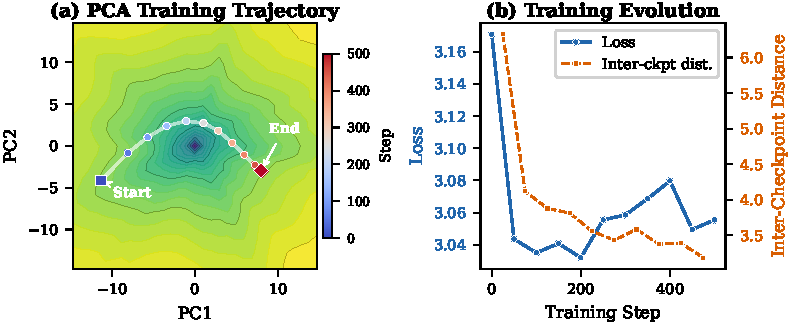
\includegraphics[width=\textwidth]{figure_4.pdf}
\caption{Training trajectory analysis of Qwen3-0.6B-Base fine-tuned for 500 steps (11 checkpoints). (a)~Trajectory-PCA (MMSP Method A): checkpoints (colored by step) project onto a smooth curved arc in the top-2 PCA plane, overlaid on the loss surface contours. PC1+PC2 capture 87.6\% of trajectory variance. (b)~Training evolution: evaluation loss (left axis) shows rapid initial improvement then plateau; inter-checkpoint parameter distance (right axis) decreases monotonically, indicating convergence.}
\label{fig:trajectory}
\end{figure}

\textbf{Decelerating dynamics.} Inter-checkpoint parameter distances decrease monotonically from 6.33 (steps 0--50) to 3.18 (steps 450--500), a $2.0\times$ deceleration consistent with convergence toward a basin center.

\textbf{Landscape stability.} Independent Tier~1 surfaces of the base and fine-tuned models show remarkable geometric stability: roughness changes by $<1\%$ (0.384 $\to$ 0.382), basin diameter widens by 5.2\% (0.328 $\to$ 0.345), and curvature ratio remains near unity (0.927 $\to$ 0.929). Fine-tuning reshapes the loss value while preserving local geometric structure.

\textbf{Anchor-point (MMSP Method B).} The interpolation between base and fine-tuned models is smooth (roughness $= 0.019$, $20\times$ lower than random-direction surfaces) with no loss barrier. The curvature ratio of $66.0{:}1$ indicates the training trajectory follows a narrow valley.

%-----------------------------------------------------------------------------
\subsection{Post-Training Effect Analysis}
\label{sec:posttraining}
%-----------------------------------------------------------------------------

We compare the officially released Qwen3-0.6B-Base against Qwen3-0.6B (post-trained with RLHF/alignment, 751M parameters) using both MMSP Methods B and C.

\textbf{RLHF fundamentally reshapes landscape geometry (Table~\ref{tab:posttraining}, Figure~\ref{fig:posttraining}).} MMSP Method C reveals a \textbf{23.3\% basin narrowing} (diameter: 0.310 $\to$ 0.238), substantially larger than fine-tuning's 5.2\% widening. Loss range decreases by 8.1\%, roughness by 3.9\%, and basin flatness by 29.3\%. The post-trained model has higher WikiText-2 loss (3.636 vs.\ 3.171), reflecting the expected perplexity-alignment trade-off.

\begin{figure}[t]
\centering
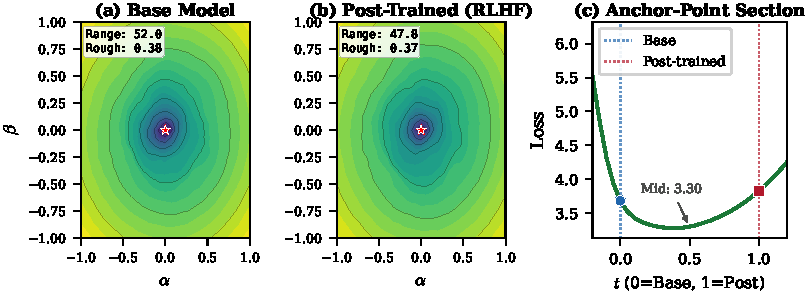
\includegraphics[width=\textwidth]{figure_5.pdf}
\caption{Post-training effect analysis: Qwen3-0.6B-Base vs.\ Qwen3-0.6B (RLHF-aligned). (a,b)~Independent Tier~1 surfaces (MMSP Method C) with matched color scales: the RLHF-aligned model shows a narrower basin (diameter $-23.3\%$) and reduced loss range ($-8.1\%$). (c)~Anchor-point 1D cross-section (MMSP Method B): smooth, barrier-free transition between base and post-trained models; midpoint loss (3.30) lies between endpoints.}
\label{fig:posttraining}
\end{figure}

\textbf{RLHF vs.\ fine-tuning: qualitatively different signatures.} The anchor-point curvature ratio is $2.98{:}1$ for RLHF (parameter distance 91.2) vs.\ $66.0{:}1$ for fine-tuning (distance 18.7). Fine-tuning follows a narrow valley along a single direction; RLHF makes broad modifications across many directions. This provides a geometric explanation for why RLHF-aligned models are more fragile to subsequent fine-tuning: a narrower basin (23.3\% smaller) is geometrically easier to escape.

\begin{table}[t]
\centering
\caption{Geometric comparison of fine-tuning (500 steps) vs.\ official RLHF post-training on Qwen3-0.6B.}
\label{tab:posttraining}
\small
\begin{tabular}{lccc}
\toprule
\textbf{Metric} & \textbf{Base} & \textbf{Fine-Tuned ($\Delta$)} & \textbf{RLHF ($\Delta$)} \\
\midrule
Parameter distance & --- & 18.71 & 91.23 \\
Eval loss & 3.171 & 3.055 ($-3.6\%$) & 3.636 ($+14.7\%$) \\
Loss range & 52.04 & 52.59 ($+1.1\%$) & 47.80 ($-8.1\%$) \\
Basin diameter & 0.310 & 0.345 ($+5.2\%$) & 0.238 ($\mathbf{-23.3\%}$) \\
Basin flatness & 2.953 & 2.411 ($-15.7\%$) & 2.089 ($-29.3\%$) \\
Anchor curv.\ ratio & --- & 66.0:1 & 2.98:1 \\
Anchor roughness & --- & 0.019 & 0.045 \\
\bottomrule
\end{tabular}
\end{table}

%-----------------------------------------------------------------------------
\subsection{Cross-Model Comparison}
\label{sec:crossmodel}
%-----------------------------------------------------------------------------

Using MMSP Method C with Tier~1 directions, we compare Qwen2.5-7B-Instruct (instruction-following), OLMo-3-7B-Think (chain-of-thought reasoning), and Qwen3-0.6B-Base (reference).

\begin{table}[t]
\centering
\caption{Cross-model landscape metrics using MMSP Method C (Tier~1, TADN, WikiText-2).}
\label{tab:crossmodel}
\small
\begin{tabular}{lcccccc}
\toprule
\textbf{Model} & \textbf{Params} & \textbf{Loss Range} & \textbf{Roughness} & \textbf{Basin Diam.} & \textbf{Curv.\ Ratio} & \textbf{Convexity} \\
\midrule
Qwen3-0.6B-Base & 596M & 52.04 & 0.384 & 0.310 & 1.060 & 0.674 \\
Qwen2.5-7B-Instruct & 7.62B & 43.86 & 0.720 & 0.252 & 0.691 & 0.573 \\
OLMo-3-7B-Think & 7.30B & 13.37 & 0.303 & 0.226 & 0.954 & 0.632 \\
\bottomrule
\end{tabular}
\end{table}

\textbf{Different training objectives produce distinct geometries (Table~\ref{tab:crossmodel}, Figure~\ref{fig:crossmodel}).} OLMo-3-7B-Think shows a much flatter WikiText-2 landscape (loss range $3.3\times$ smaller than Qwen~7B), reflecting its reasoning-focused training which distributes probability across thinking tokens rather than concentrating on next-token prediction. Despite similar parameter counts ($\sim$7B), the two models exhibit clearly distinct geometric profiles.

\begin{figure}[t]
\centering
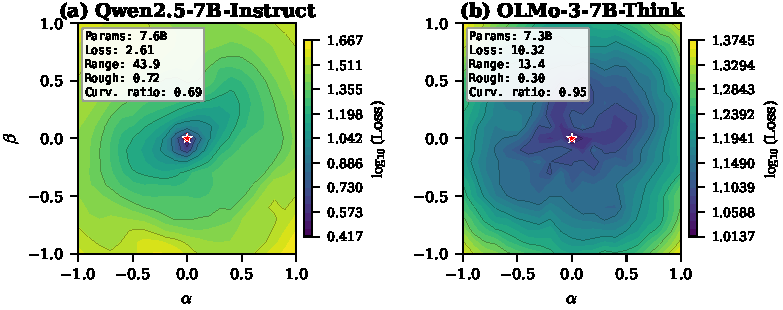
\includegraphics[width=\textwidth]{figure_6.pdf}
\caption{Cross-model comparison of 7B-parameter models using MMSP Method C (Tier~1, TADN). (a)~Qwen2.5-7B-Instruct: instruction-following model with loss range 43.9 and higher roughness (0.72). (b)~OLMo-3-7B-Think: reasoning-focused model with dramatically flatter landscape (loss range 13.4, roughness 0.30). Despite similar parameter counts, different training objectives produce distinct landscape geometries.}
\label{fig:crossmodel}
\end{figure}

\textbf{Basin diameter decreases with model size:} 0.310 (0.6B) $\to$ 0.252 (7B Qwen) $\to$ 0.226 (7B OLMo), suggesting larger models converge to sharper minima in TADN-normalized space. Convexity also decreases with scale (0.674 $\to$ 0.573), indicating more non-convex structure in larger models.

\textbf{Scalability.} Tier~1 analysis of 7B models completes in $\sim$79 minutes on a single A100-40GB. Tier~2 (gradient PCA) for 7B models exceeds 40GB memory due to gradient storage requirements, establishing the current scalability boundary.

%-----------------------------------------------------------------------------
\subsection{Dataset Sensitivity and Robustness}
\label{sec:dataset}
%-----------------------------------------------------------------------------

To verify that landscape geometry is a model property rather than a data artifact, we evaluate Qwen3-0.6B-Base with identical TADN-normalized directions across five datasets (Table~\ref{tab:dataset}).

\begin{table}[t]
\centering
\caption{Dataset sensitivity analysis for Qwen3-0.6B-Base (Tier~1, TADN, 31$\times$31 grid).}
\label{tab:dataset}
\small
\begin{tabular}{lccccc}
\toprule
\textbf{Dataset} & \textbf{Base Loss} & \textbf{Loss Range} & \textbf{Roughness} & \textbf{Basin Diam.} & \textbf{Curv.\ Ratio} \\
\midrule
WikiText-2 (test) & 3.000 & 52.04 & 0.384 & 0.310 & 1.060 \\
WikiText-2 (train) & 3.231 & 51.95 & 0.380 & 0.301 & 1.050 \\
WikiText-2 (val) & 2.753 & 52.55 & 0.384 & 0.291 & 1.052 \\
Synthetic Code & 0.801 & 54.37 & 0.433 & 0.281 & 1.035 \\
Structured/Tabular & 1.325 & 54.09 & 0.424 & 0.345 & 1.066 \\
\midrule
\textbf{Mean $\pm$ Std (all 5)} & --- & 52.98 $\pm$ 1.04 & 0.401 $\pm$ 0.022 & 0.306 $\pm$ 0.021 & 1.053 $\pm$ 0.011 \\
\textbf{CV (\%)} & --- & 2.0\% & 5.5\% & 7.0\% & 1.0\% \\
\bottomrule
\end{tabular}
\end{table}

Baseline losses vary by $4\times$ across domains (0.80--3.23), yet loss range remains within 52--54 (CV $= 2.0\%$) and curvature ratio within 1.04--1.07 (CV $= 1.0\%$). The landscape geometry captures intrinsic model structure rather than data-specific loss values. Even 512 tokens (2 chunks) produce loss ranges within 2\% of the full-data value, demonstrating that accurate landscape characterization requires minimal evaluation data.

%=============================================================================
\section{Discussion}
\label{sec:discussion}
%=============================================================================

\textbf{PFI as a standard for visualization quality.} Our results show that random projections for LLMs capture essentially zero spectral energy (PFI-S $\approx 10^{-9}$), confirming theoretical predictions. PFI enables practitioners to make \emph{informed} decisions about the cost--quality trade-off: Tier~2 provides $8{,}500\times$ improvement over random at the cost of $\sim$100 gradient computations, while Tier~3 provides an additional $4.9\times$ using $\sim$60 HVPs. We recommend reporting PFI alongside any loss landscape visualization.

\textbf{Geometric signatures of alignment.} The finding that RLHF narrows the basin by 23.3\% while fine-tuning widens it by 5.2\% provides geometric evidence for the empirically observed alignment fragility phenomenon~\citep{chen2025unveiling}: a narrower basin is geometrically easier to escape through adversarial fine-tuning. The qualitative difference between fine-tuning (narrow valley, anisotropy 66:1) and RLHF (broad modification, anisotropy 3:1) reflects fundamentally different optimization dynamics in parameter space.

\textbf{Scalability and limitations.} Tier~1 (Random+TADN) scales to any model that fits in GPU memory for inference. Tier~2/3 are currently limited to $\sim$1B parameters on 40GB hardware due to gradient/Hessian memory requirements. Memory-efficient extensions---streaming PCA, gradient compression, randomized Lanczos methods---could extend the practical boundary. Even at Tier~1, the framework produces consistent, reproducible geometric characterizations (CV $< 1\%$ for loss range) that enable meaningful cross-model comparison.

\textbf{The 2D projection ceiling.} Even the optimal 2D projection captures at most $\sim$0.02\% of total Hessian spectral energy (Tier~3 PFI-S $= 1.90 \times 10^{-4}$). PFI makes this limitation explicit and quantifiable, enabling honest communication about what any 2D visualization does---and does not---reveal about the true high-dimensional geometry.

%=============================================================================
\section{Conclusion}
\label{sec:conclusion}
%=============================================================================

We presented LLMScape, a framework for faithful and scalable loss landscape visualization of large language models. LLMScape introduces five contributions---TADN, SHIDS, PFI, MMSP, and an efficient computation pipeline---that together address the fundamental challenges of visualizing loss landscapes at LLM scale. TADN achieves provably perfect scale invariance under transformer symmetries. PFI provides the first quantitative metric for visualization faithfulness, revealing a $41{,}400\times$ quality difference between random and Hessian-informed projections. The framework scales to 7B parameters, a $700\times$ increase over prior visualization work.

Applied to training dynamics and post-training analysis, LLMScape reveals concrete geometric insights: fine-tuning follows connected, narrow valleys in parameter space ($66{:}1$ curvature anisotropy) while preserving landscape geometry, whereas RLHF alignment fundamentally reshapes the basin---narrowing it by 23.3\%---providing a geometric perspective on the empirically observed fragility of aligned models. Different model families exhibit distinct landscape geometries tied to their training objectives rather than their parameter counts.

We believe that reporting PFI alongside loss landscape visualizations should become standard practice, and that the geometric perspective on LLM training provided by LLMScape complements the prevailing benchmark-driven evaluation paradigm. Future work includes memory-efficient extensions for Tier~2/3 at 7B+ scale, connecting landscape geometry to downstream task performance, and PFI-guided direction optimization.

\paragraph{Limitations.}
Tier~2 (gradient PCA) and Tier~3 (Hessian eigenvectors) are currently limited to $\sim$1B parameters on single 40GB GPUs due to gradient and HVP memory requirements. Even the optimal 2D projection captures at most $\sim$0.02\% of total Hessian spectral energy (PFI-S $= 1.90 \times 10^{-4}$ for Tier~3), a fundamental consequence of projecting from $d \approx 600$M dimensions to 2D. Our invariance analysis targets SwiGLU-based transformers; other architectures (e.g., MoE, GeLU FFN) exhibit different symmetries that may require additional normalization units. The interpretation of basin narrowing as evidence for alignment fragility is correlational; establishing a causal link between landscape geometry and alignment robustness remains an open question.

\paragraph{Broader Impact.}
LLMScape is a diagnostic and analysis tool that improves scientific understanding of LLM training dynamics. The geometric perspective on alignment (e.g., basin narrowing under RLHF) could help improve the safety and robustness of aligned models by guiding the design of alignment procedures that produce wider, more robust basins. We do not foresee significant negative societal impacts from this work.


%=============================================================================
% References
%=============================================================================
\bibliographystyle{plainnat}
\bibliography{references}

%=============================================================================
% Appendix
%=============================================================================
\newpage
\appendix

\section{Proof of Proposition~\ref{prop:tadn_invariance}}
\label{app:proof_tadn}

\begin{proof}
Under the rescaling $W_{\mathrm{up},j}' = c_j W_{\mathrm{up},j}$ and $W_{\mathrm{down}}'^{(:,j)} = c_j^{-1} W_{\mathrm{down}}^{(:,j)}$, TADN's per-neuron normalization produces:
\begin{align}
\hat{d}'_{\mathrm{up},j} &= \frac{d_{\mathrm{up},j}}{\|d_{\mathrm{up},j}\|_F} \cdot \|c_j W_{\mathrm{up},j}\|_F = c_j \cdot \frac{d_{\mathrm{up},j}}{\|d_{\mathrm{up},j}\|_F} \cdot \|W_{\mathrm{up},j}\|_F = c_j \hat{d}_{\mathrm{up},j} \\
\hat{d}'_{\mathrm{down},j} &= \frac{d_{\mathrm{down},j}}{\|d_{\mathrm{down},j}\|_F} \cdot \|c_j^{-1} W_{\mathrm{down},j}\|_F = c_j^{-1} \hat{d}_{\mathrm{down},j}
\end{align}

The perturbed SwiGLU FFN output for neuron $j$ under the rescaled parameterization is:
\begin{align}
\mathrm{FFN}'_j &= (c_j^{-1} W_{\mathrm{down},j} + \alpha c_j^{-1} \hat{d}_{\mathrm{down},j}) \cdot \mathrm{swish}(W_{\mathrm{gate},j} x) \cdot (c_j W_{\mathrm{up},j} + \alpha c_j \hat{d}_{\mathrm{up},j}) x \\
&= (W_{\mathrm{down},j} + \alpha \hat{d}_{\mathrm{down},j}) \cdot \mathrm{swish}(W_{\mathrm{gate},j} x) \cdot (W_{\mathrm{up},j} + \alpha \hat{d}_{\mathrm{up},j}) x = \mathrm{FFN}_j
\end{align}

Since this holds for every neuron $j$ in every layer, the total network output is identical: $L(\theta' + \alpha \hat{\mathbf{d}}') = L(\theta + \alpha \hat{\mathbf{d}})$.
\end{proof}

\section{Proof of Theorem~\ref{thm:pfi}}
\label{app:proof_pfi}

\begin{proof}
\textbf{(i)} Since $H^2$ is positive semi-definite, $\hat{\mathbf{d}}_i^\top H^2 \hat{\mathbf{d}}_i \geq 0$ for all unit vectors, so $\mathrm{PFI\text{-}S} \geq 0$. For the upper bound, $\hat{\mathbf{d}}_i^\top H^2 \hat{\mathbf{d}}_i \leq \lambda_{\max}(H^2) = \lambda_1^2$, and $\mathrm{tr}(H^2) \geq \lambda_1^2 + \lambda_2^2$, so $\mathrm{PFI\text{-}S} \leq 2\lambda_1^2 / (\lambda_1^2 + \lambda_2^2) \leq 1$ when $\lambda_2 \geq 0$ (which holds since $H^2$ eigenvalues are non-negative).

\textbf{(ii)} By the Courant--Fischer min-max theorem, $\max_{U: \dim U = 2} \sum_{i=1}^{2} \hat{\mathbf{d}}_i^\top H^2 \hat{\mathbf{d}}_i = \lambda_1(H^2) + \lambda_2(H^2) = \lambda_1^2 + \lambda_2^2$, achieved when $\hat{\mathbf{d}}_1, \hat{\mathbf{d}}_2$ are the top-2 eigenvectors of $H^2$ (equivalently, of $|H|$, which shares eigenvectors with $H$).

\textbf{(iii)} For a random unit vector $\hat{\mathbf{d}} \sim \mathrm{Uniform}(S^{d-1})$: $\mathbb{E}[\hat{\mathbf{d}}^\top H^2 \hat{\mathbf{d}}] = \frac{1}{d}\mathrm{tr}(H^2)$. For two orthogonal random unit vectors: $\mathbb{E}[\mathrm{PFI\text{-}S}] = \frac{2}{d} \cdot \frac{\mathrm{tr}(H^2)}{\mathrm{tr}(H^2)} = \frac{2}{d}$.
\end{proof}

\section{Additional Ablation Results}
\label{app:ablations}

\textbf{Grid resolution independence.} Loss range is identical at 11$\times$11 through 51$\times$51 (52.04 at all resolutions). Roughness decreases with resolution (1.663 $\to$ 0.219), and basin diameter converges by 21$\times$21 (within 3\% of the 51$\times$51 value). We recommend 21$\times$21 for loss range and basin diameter, 31$\times$31+ for roughness.

\textbf{Evaluation data size.} Even 512 tokens (2 chunks) capture the loss range within 2\% of the 12,800-token value. Basin diameter is identical across all sizes (0.319). This is a practically important finding: accurate landscape characterization requires minimal data.

\textbf{PCA sample size.} Gradient PCA subspace angles drop from 80.7$^{\circ}$ (N=30 vs.\ N=20) to 26.2$^{\circ}$ (N=50 vs.\ N=30), showing initial convergence around N=50. However, subspace angles remain moderate at N=100 (53.4$^{\circ}$), indicating the effective dimensionality of the gradient distribution is high for 596M-parameter models.

\section{Hessian Eigenvector Analysis}
\label{app:hessian}

For Qwen3-0.6B-Base, power iteration converges in 7--8 iterations, yielding $\lambda_1 = 14{,}329$ and $\lambda_2 = 8{,}298$ (spectral gap ratio $\lambda_1/\lambda_2 = 1.73$). The characteristic curvature length $\ell_{\mathrm{char}} = 1/\sqrt{\lambda_1} = 0.00835$ is $120\times$ smaller than the Tier~1 grid range, confirming that Hessian eigenvectors probe fundamentally different curvature scales. Total computation time: $\sim$2 minutes on a single A100-40GB.

\end{document}
